\chapter{結論}
\section{AIによる楽曲制作の結果}
\subsection{モデルによる生成結果の違い}
\begin{figure}[h]
    \begin{screen}
    \begin{center}
        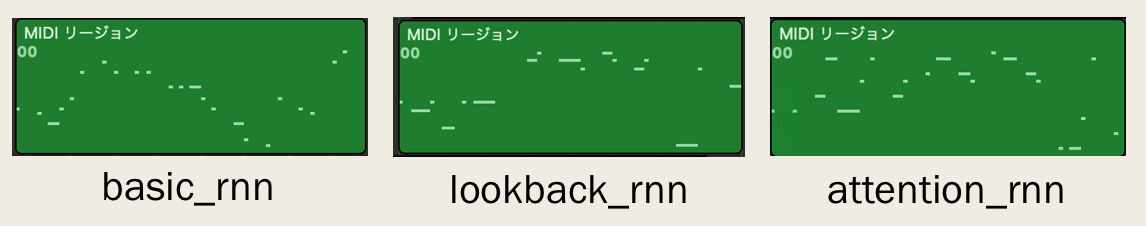
\includegraphics[scale=0.68, clip]{./img/model.png}
        \caption{学習モデルごとの生成結果}
        \label{fig:学習モデルごとの生成結果}
    \end{center}
    \end{screen}
\end{figure}
\newpage
\subsection{学習回数による生成結果の違い}
\begin{figure}[h]
    \begin{screen}
    \begin{center}
        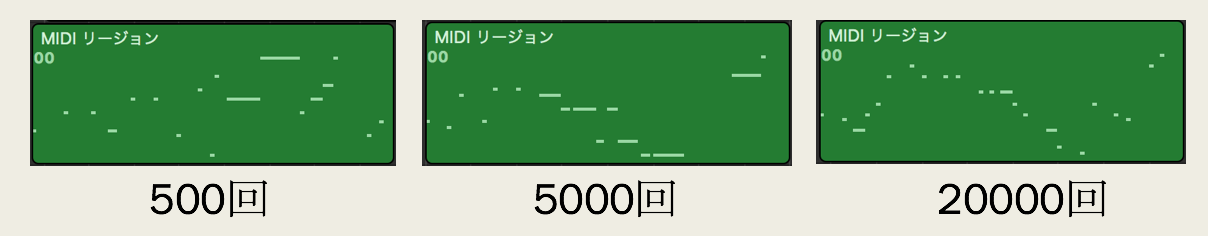
\includegraphics[scale=0.68, clip]{./img/basicMIDI.png}
        \caption{basic\_rnnによる学習回数ごとの生成結果}
        \label{fig:basic_rnnによる学習回数ごとの生成結果}
    \end{center}
    \end{screen}
\end{figure}
\begin{figure}[h]
    \begin{screen}
    \begin{center}
        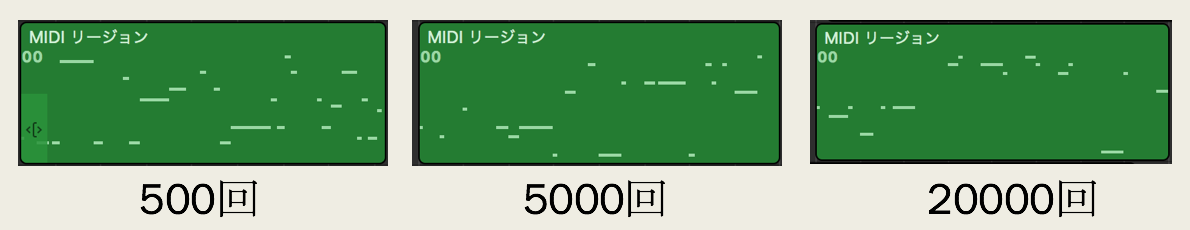
\includegraphics[scale=0.68, clip]{./img/lookbackMIDI.png}
        \caption{lookback\_rnnによる学習回数ごとの生成結果}
        \label{fig:lookback_rnnによる学習回数ごとの生成結果}
    \end{center}
    \end{screen}
\end{figure}
\begin{figure}[h]
    \begin{screen}
    \begin{center}
        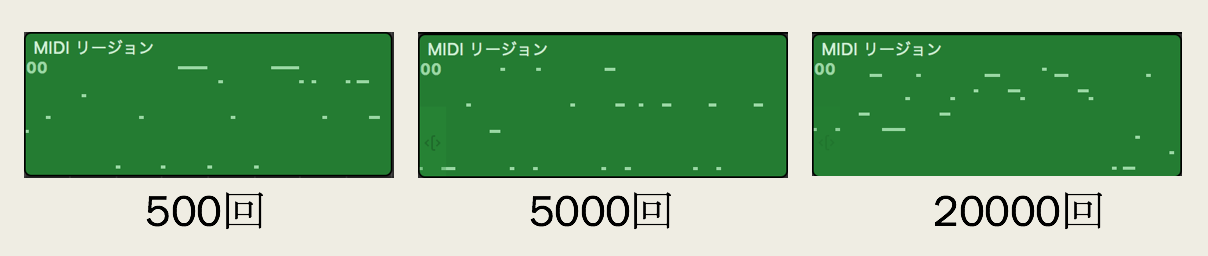
\includegraphics[scale=0.68, clip]{./img/attentionMIDI.png}
        \caption{attention\_rnnによる学習回数ごとの生成結果}
        \label{fig:attention_rnnによる学習回数ごとの生成結果}
    \end{center}
    \end{screen}
\end{figure}
\newpage
\subsection{ノード数による生成結果の違い}
\begin{figure}[h]
    \begin{screen}
    \begin{center}
        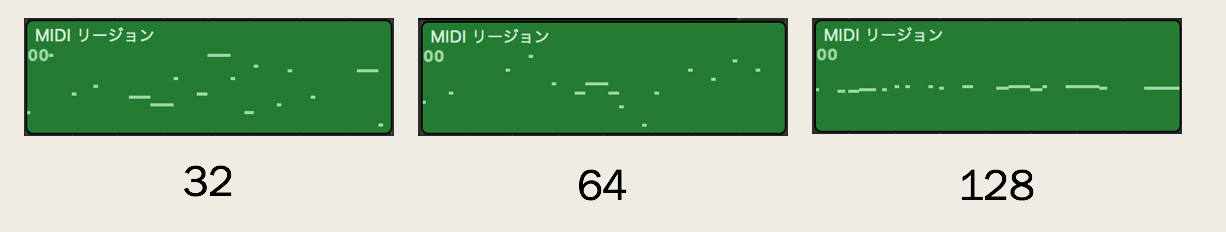
\includegraphics[scale=0.68, clip]{./img/nodo.png}
        \caption{ノード数ごとの生成結果}
        \label{fig:ノード数ごとの生成結果}
    \end{center}
    \end{screen}
\end{figure}
\newpage
\section{調査結果}
 楽曲制作に関して有用な条件をアンケート形式で調査した.調査方法はMelodyRNNによる三種の生成結果,学習回数ごとの生成結果,ノード数ごとの生成結果
のそれぞれの項目から一番良いと思うものを選択してもらう形式を取った.以下に結果を示す.
\begin{figure}[h]
    \begin{screen}
    \begin{center}
        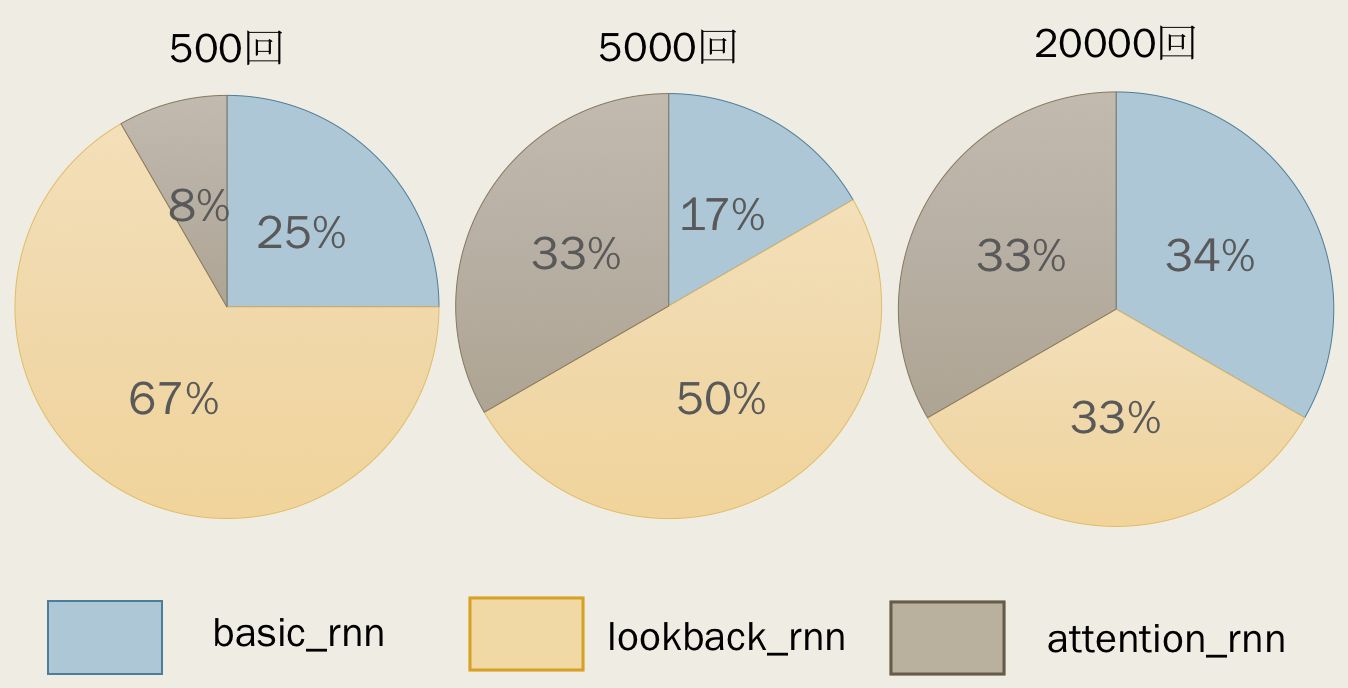
\includegraphics[scale=0.5, clip]{./img/glaph1.png}
        \caption{学習回数ごとの各モデルの調査結果}
        \label{fig:学習回数ごと各モデルの調査結果}
    \end{center}
    \end{screen}
\end{figure}
\begin{figure}[h]
    \begin{screen}
    \begin{center}
        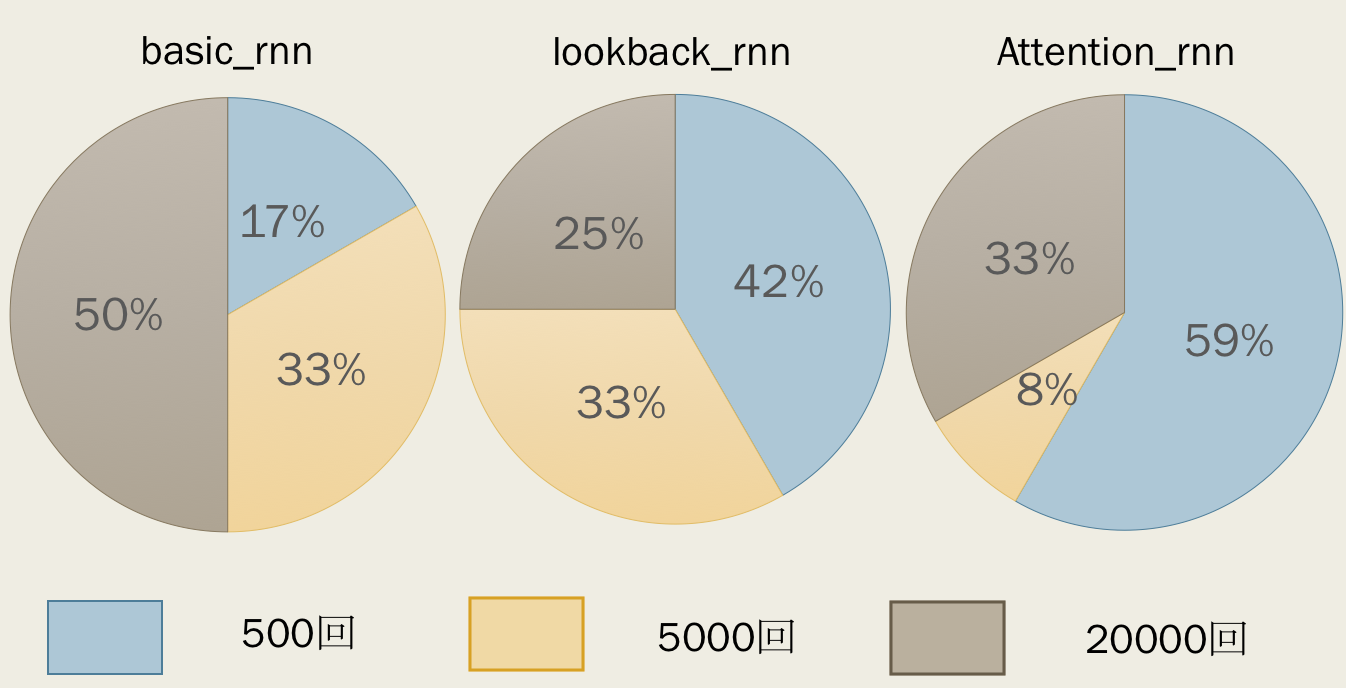
\includegraphics[scale=0.5, clip]{./img/glaph2.png}
        \caption{各モデルごと学習回数の調査結果}
        \label{fig:各モデルごとの学習回数の調査結果}
    \end{center}
    \end{screen}
\end{figure}
\begin{figure}[h]
    \begin{screen}
    \begin{center}
        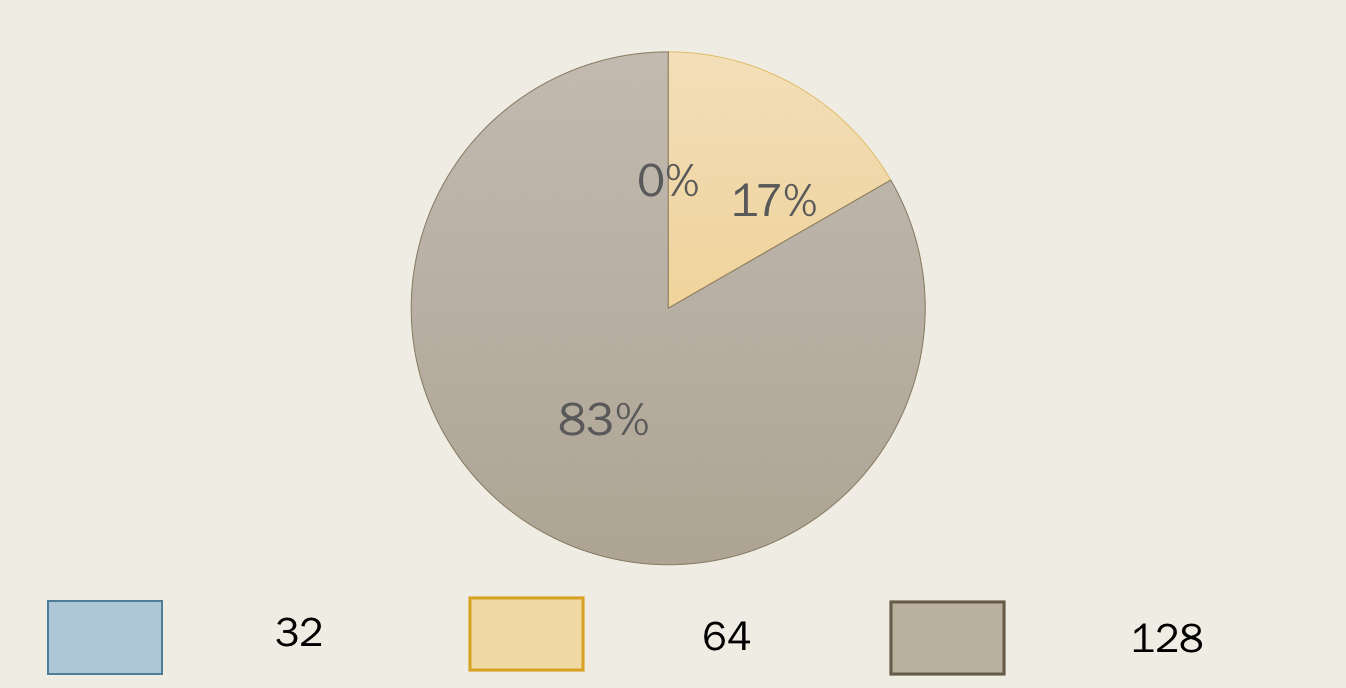
\includegraphics[scale=0.5, clip]{./img/glaph3.png}
        \caption{ノード数ごとの調査結果}
        \label{fig:ノード数の調査結果}
    \end{center}
    \end{screen}
\end{figure}

\newpage
\section{今後の課題}
今回,様々な条件で楽曲を制作した.特に学習回数を大きくすると楽曲の精度は高まった.しかし音階やスケールは理解できているようだが,メロディに関してはあまり良いものとは言えなかった.要因としては学習に用いる楽曲が少なかったことや学習回数がまだ足りなかったことがあげられる.\\
